\documentclass[11pt]{article}
% -- Formato
% -- Formato realizado en febrero de 2024
% -- Corre sin problema en TeX Live 2023
% -- Adapta correctamente normas APA con BibLaTeX

% -- Paquetes básicos
\usepackage[spanish,es-nolists]{babel}
\usepackage[utf8]{inputenc}
\usepackage[noblocks]{authblk} % Para poner afiliación
    \renewcommand\Authsep{; }
    \renewcommand\Authand{; }
    \renewcommand\Authands{; }
    \renewcommand\Affilfont{\small}
    \setcounter{Maxaffil}{1}
\usepackage{xcolor}
\usepackage{booktabs}
\usepackage{float}
\usepackage{graphicx}
\usepackage[colorlinks,allcolors=.]{hyperref}
\usepackage[a4paper, hmargin=2cm, vmargin=4cm]{geometry}
\usepackage{iftex}
\usepackage{silence}

% -- Formato de título
\usepackage{titling}
\pretitle{\vspace*{-2cm}\begin{center}\bfseries\LARGE}
\posttitle{\end{center}}

% -- Tipo de letra
\ifPDFTeX % LaTeX y pdfLaTeX
    \RequirePackage[defaultfam,tabular,lining]{montserrat}
        \renewcommand*\oldstylenums[1]{{\fontfamily{Montserrat-TOsF}\selectfont #1}}
    \RequirePackage[OT1]{eulervm}
    \renewcommand{\labelitemi}{$\bullet$}
    \DeclareMathSizes{10}{10.78}{7}{7}
\else % XeLaTeX
    \RequirePackage[OT1]{eulervm}
    \RequirePackage{fontspec}
    \setmainfont{montserrat}
    \DeclareSymbolFont{operators}{\encodingdefault}{\familydefault}{m}{n}
    \DeclareMathSizes{10}{10.78}{7}{7}
    \renewcommand{\labelitemi}{$\bullet$}
\fi
\WarningFilter{latexfont}{Font shape  `T1/cmtt/regular/n'}
\WarningFilter{latexfont}{Some font shapes were not available, defaults substituted.}

% -- Fondo
\WarningsOff[everypage]
\usepackage[pages=all]{background}
\backgroundsetup{
    scale=1,color=black,opacity=1,angle=0,
    hshift=0mm,
    vshift=0mm,
    contents={
\includegraphics[width=210mm]{HojaMembretada.pdf}}
}

% -- Formato de bibliografía
\usepackage{csquotes}
\usepackage[backend=biber, style=apa]{biblatex}
% -- Adaptar apa al español (2023)
    \makeatletter
    \DefineBibliographyExtras{spanish}{ 
        % Código para corregir &
        \setcounter{smartand}{1}
    	\let\lbx@finalnamedelim=\lbx@es@smartand
    	\let\lbx@finallistdelim=\lbx@es@smartand
        % Código para corregir coma final
        \renewcommand*{\apablx@ifrevnameappcomma}[2]{#2}
        \let\finalandcomma=\empty
    }
    \makeatother
    \setlength{\bibhang}{\parindent}
% -- Fin de adaptar apa al español (2023)

% -- Formato leyendas
\usepackage[font={small},labelfont={bf,small},
    justification=centerlast,tablename=Tabla]{caption}
\usepackage{listings}
    \renewcommand{\lstlistingname}{Código}

% -- Formato Código
\lstdefinestyle{mystyle}{
    backgroundcolor=\color{gray!20},   
    commentstyle=\color{teal},
    keywordstyle=\color{purple},
    stringstyle=\color{violet},
    basicstyle=\ttfamily\footnotesize,
    breaklines=true,                 
    captionpos=b,                    
    showstringspaces=false,
    linewidth=0.95\linewidth,
    literate={\ \ }{{\ }}1,
    xleftmargin=0.05\linewidth,
}
\lstset{style=mystyle}

% -- Espacio
\setlength{\parskip}{0.4\baselineskip}
\renewcommand{\baselinestretch}{1.2}


\usepackage[many]{tcolorbox}
\usepackage{amsthm}
\definecolor{colordef}{cmyk}{0.81,0.62,0.00,0.22}
\newtheoremstyle{estiloteorema}%
    {9pt}{9pt}{}{0pt}
    {\bfseries\color{\tcb@@color}}
    {}{ }
    {\textsc{\thmname{#1}\thmnumber{ #2}}\thmnote{: #3}.}
\makeatletter
%%  Keys temporales: |tipo|,|color|, |contador| e |icóno|.
\def\tcb@@tipo{}
    \tcbset{ tipo/.code = {\def\tcb@@tipo{#1} } }
\def\tcb@@contador{}
    \tcbset{ contador/.code = {\def\tcb@@contador{#1} } }
\def\tcb@@color{colordef}
    \tcbset{ color/.code = {\def\tcb@@color{#1} } }
\def\tcb@@icono{{\large\faWarning}}
    \tcbset{ icono/.code = {\def\tcb@@icono{#1} } }
\tcbset{ recuadrost/.style ={
    before skip=10pt,arc=0mm,breakable,enhanced,
    colback=\tcb@@color!7,colframe=\tcb@@color,
    boxrule=0pt,leftrule=2pt,
    top=0.5mm,bottom=0.5mm,left=2mm,right=2mm,
    fontupper=\normalsize,
    % parbox=false
    }
    }
\makeatother
\newtheorem{ejer}{Ejercicio}
    \tcolorboxenvironment{ejer}{%
        color=colordef,recuadrost,colback=colordef!7,drop fuzzy shadow
    }

% -- Paquetes adicionales
\usepackage{amsmath,amssymb}
\usepackage{enumitem}



% -- Comandos extra


% -- Datos
\title{Álgebra Lineal y la Ciencia de Datos}
\author{Andrés Merino}
\affil{Carrera de Ciencia de Datos}
\date{\today}

% --- Archivo de bibliografía
\addbibresource{01 Referencias.bib}

%%%%%%%%%%%%%%%%%%%%%%%%%%%%%%%%%%%%%%%%
\begin{document}

%%%%%%%%%%%%%%%%%%%%%%%%%%%%%%%%%%%%%%%%
\maketitle


%%%%%%%%%%%%%%%%%%%%%%%%%%%%%%%%%%%%%%%%
\section{Introducción}
%%%%%%%%%%%%%%%%%%%%%%%%%%%%%%%%%%%%%%%%

Lorem ipsum dolor sit amet, consectetuer adipiscing elit. Ut purus elit, vestibulum ut, placerat ac, adipiscing vitae, felis. Curabitur dictum gravida mauris. Namarcu libero, nonummy eget, consectetuer id, vulputate a, magna. Donec vehicula augue eu neque. Pellentesque habitant morbi tristique senectus et netus et malesuada fames ac turpis egestas. Mauris ut leo. Cras viverra metus rhoncus sem. Nulla et lectus vestibulum urna fringilla ultrices. Phasellus eu tellus sit amet tortor gravida placerat. Integer sapien est, iaculis in, pretium quis, viverra ac, nunc. Praesent eget sem vel leo ultrices bibendum. Aenean faucibus. Morbi dolor nulla, malesuada eu, pulvinar at, mollis ac, nulla. Curabitur auctor semper nulla. Donec varius orci eget risus. Duis nibh mi, congue eu, accumsan eleifend, sagittis quis, diam. Duis eget orci sit amet orci dignissim rutrum.

Nam dui ligula, fringilla a, euismod sodales, sollicitudin vel, wisi. Morbi auctor lorem non justo. Nam lacus libero, pretium at, lobortis vitae, ultricies et, tellus. Donec aliquet, tortor sed accumsan bibendum, erat ligula aliquet magna, vitae ornare odio metus a mi. Morbi ac orci et nisl hendrerit mollis. Suspendisse ut massa. Cras nec ante. Pellentesque a nulla. Cum sociis natoque penatibus et magnis dis parturient montes, nascetur ridiculus mus. Aliquam tincidunt urna. Nulla ullamcorper vestibulum turpis. Pellentesque cursus luctus mauris

%%%%%%%%%%%%%%%%%%%%%%%%%%%%%%%%%%%%%%%%
\section{Figuras y Tablas}
%%%%%%%%%%%%%%%%%%%%%%%%%%%%%%%%%%%%%%%%

Las tablas e imágenes que aparezcan en el documento, siempre deben ser referenciadas, se deben hacer referencia a ellas con enlaces, por ejemplo: en la Figura \ref{fig:01} y en la Tabla \ref{tab:01} se pueden apreciar los resultados.

\begin{figure}[H]
    \centering
    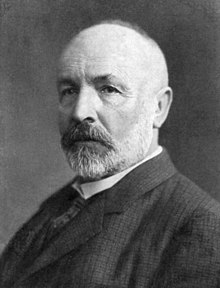
\includegraphics[width=0.4\textwidth]{01 Figuras/fig01.jpg}
    \caption{Leyenda de la figura.}
    \label{fig:01}
\end{figure}

Para la composición de tablas, la letra siempre debe ser de tamaño menor a la del resto del texto y se recomienda optar por el siguiente formato:

\begin{table}[H]
    \centering\small
    \begin{tabular}{@{}ccc@{}}
    \toprule
        \textbf{Fórmula} & \textbf{Prueba 1} & \textbf{Prueba 2} \\ 
    \midrule
        Compuesto 1 & $38.4$  &  $6.32$\\ 
        Compuesto 2 & $16.6$ & $12.5$ \\ 
    \bottomrule
    \end{tabular}
    \caption{Resultados de la experimentación de distintas substancias.}
    \label{tab:01}
\end{table}

Las tablas, al igual que las figuras, siempre deben poseer una leyenda. Este hace uso del paquete \texttt{booktabs} que mejora la presentación de las mismas. También se pueden ingresar código como el que se muestra en el Código \ref{lst:01}.

\begin{lstlisting}[language=Python,caption={Ejemplo de código.},label={lst:01},captionpos=b]
# Ordenamiento por burbuja
def OrdenBurbuja(a):
    for i in range(len(a)-2):
        for j in range(len(a)-i-1):
            if a[j] > a[j+1]:
                a[j],a[j+1] = a[j+1],a[j]
    print("Se ha ordenado la lista.")
    return a
\end{lstlisting}

%%%%%%%%%%%%%%%%%%%%%%%%%%%%%%%%%%%%%%%%
\section{Conclusiones}
%%%%%%%%%%%%%%%%%%%%%%%%%%%%%%%%%%%%%%%%

\begin{itemize}[leftmargin=*]
\item 
    Lorem ipsum dolor sit amet, consectetuer adipiscing elit. Ut purus elit, vestibulum ut, placerat ac, adipiscing vitae, felis. Curabitur dictum gravida mauris. Namarcu libero, nonummy eget, consectetuer id, vulputate a, magna. Donec vehicula augue eu neque. Pellentesque habitant morbi tristique senectus et netus et malesuada fames ac turpis egestas. Mauris ut leo. Cras viverra metus rhoncus sem. Nulla et lectus vestibulum urna fringilla ultrices. Phasellus eu tellus sit amet tortor gravida placerat. Integer sapien est, iaculis in, pretium quis, viverra ac, nunc. Praesent eget sem vel leo ultrices bibendum. Aenean faucibus. Morbi dolor nulla, malesuada eu, pulvinar at, mollis ac, nulla. Curabitur auctor semper nulla. Donec varius orci eget risus. Duis nibh mi, congue eu, accumsan eleifend, sagittis quis, diam. Duis eget orci sit amet orci dignissim rutrum.

\item
    Nam dui ligula, fringilla a, euismod sodales, sollicitudin vel, wisi. Morbi auctor lorem non justo. Nam lacus libero, pretium at, lobortis vitae, ultricies et, tellus. Donec aliquet, tortor sed accumsan bibendum, erat ligula aliquet magna, vitae ornare odio metus a mi. Morbi ac orci et nisl hendrerit mollis. Suspendisse ut massa. Cras nec ante. Pellentesque a nulla. Cum sociis natoque penatibus et magnis dis parturient montes, nascetur ridiculus mus. Aliquam tincidunt urna. Nulla ullamcorper vestibulum turpis. Pellentesque cursus luctus mauris
\end{itemize}

%%%%%%%%%%%%%%%%%%%%%%%%%%%%%%%%%%%%%%%%
\section{Bibliografía y citas}
%%%%%%%%%%%%%%%%%%%%%%%%%%%%%%%%%%%%%%%%

La bibliografía debe incluirse mediante un archivo \texttt{.bib}. El estilo bibliográfico a usar es APA séptima edición. Para las citas puede utilizar los siguientes comandos según sea adecuado:
\begin{itemize}
\item 
    Cita completa entre paréntesis \verb"\parencite{ }": \parencite{stewartpre}
\item
    Cita completa año entre paréntesis \verb"\textcite{ }": \textcite{stewartpre}
\item 
    Cita completa sin paréntesis \verb"\cite{ }": \cite{stewartpre}
\item
    Cita de autor \verb"\citeauthor{ }": \citeauthor{stewartpre}
\item
    Cita de año \verb"\citeyear{ }": \citeyear{stewartpre}
\item 
    Cita con opciones extras \verb"\parencite[ ][ ]{ }": \parencite[ver][p. 66]{stewartpre}
\end{itemize}

%%%%%%%%%%%%%%%%%%%%%%%%%%%%%%%%%%%%%%%%
\subsection{Ejemplos}

Nam dui ligula, fringilla a, euismod sodales, sollicitudin vel, wisi. Morbi auctor lorem non justo. Nam lacus libero, pretium at, lobortis vitae, ultricies et, tellus. Donec aliquet, tortor sed accumsan bibendum, erat ligula aliquet magna.

Según \textcite{stewartpre}, ``la forma más importante de visualizar una función es por medio de su gráfica'' (p. 152). Además, sabemos que ``la gráfica de una función $f$ da un retrato del comportamiento'' \parencite[p. 153]{stewartpre}. Por otro lado, una función se dice lineal porque su gráfica representa una recta \parencite{stewartpre}. Finalmente, según \textcite{stewartpre}:
\begin{quote}
    Por lo general consideramos funciones para las cuales los conjuntos $A$ y $B$ son conjuntos de números reales. El símbolo $f(x)$ se lee “$f$ de $x$” o “$f$ en $x$” y se denomina valor de $f$ en $x$, o la imagen de $x$ bajo $f$. El conjunto $A$ recibe el nombre de dominio de la función. El rango de $f$ es el conjunto de todos los valores posibles de $f(x)$ cuando $x$ varía en todo el dominio. (p. 125)
\end{quote}

De otra manera:
\begin{quote}
    Por lo general consideramos funciones para las cuales los conjuntos $A$ y $B$ son conjuntos de números reales. El símbolo $f(x)$ se lee “$f$ de $x$” o “$f$ en $x$” y se denomina valor de $f$ en $x$, o la imagen de $x$ bajo $f$. El conjunto $A$ recibe el nombre de dominio de la función. El rango de $f$ es el conjunto de todos los valores posibles de $f(x)$ cuando $x$ varía en todo el dominio. \parencite[p. 125]{stewartpre}
\end{quote}

%%%%%%%%%%%%%%%%%%%%%%%%%%%%%%%%%%%%%%%%
\nocite{*}
\printbibliography

\end{document}

